\section{Wprowadzenie teoretyczne}

\epigraph{There is nothing so practical as a good theory.}{Lewin Kurt}
%\epigraph{Nie ma osobnej ani teorii, ani praktyki inżynierskiej, jest tylko wspólna sztuka inżynierska.}{prof. Jan Oderfeld}

Przygotowując się do projektu o charakterze fizycznym, ważne jest, aby przed rozpoczęciem prac programistycznych dokonać dokładnego przeglądu wiedzy domenowej. Chcąc uzyskać wyniki jakościowe zgodne ze zjawiskami występującymi w rzeczywistości, należy zorientować się, czy dla implementowanych zjawisk znane i~wykorzystywane są modele fizyczne oraz, czy można w sposób zwięzły zbudować na ich podstawie model matematyczny. Dodatkowo w projekcie o charakterze ogólnym pożądane jest, aby wykorzystane modele były modelami fenomenologicznymi, tj. takimi, w których zależności wynikają z podstawowych praw fizyki, a każdemu z~parametrów można przypisać pewną interpretację fizyczną. Odrzucając powyższe podejście i opracowując projekt w oparciu o intuicję programisty, mogłoby się okazać, że rezultaty otrzymywane są w sposób nieprzewidywalny, a cały projekt posiada jedynie walory estetyczne.\\

Celem tego rozdziału jest przybliżenie wiedzy domenowej, która została wykorzystana podczas realizacji tego projektu. Szczegółowo omówiony został model dynamiki BSP, sterowanie BSP oraz nawigacja. Drugą część rozdziału stanowi teoretyczny opis elementów grafiki komputerowej, wykorzystanych podczas implementacji wizualizacji. Przedstawione zagadnienia zostaną zaprezentowane w sposób umożliwiający ich zrozumienie oraz późniejszą implementację, lecz bez dowodów poprawności. Brak formalności zostanie natomiast zrekompensowany poprzez wskazanie odpowiednich źródeł naukowych.

\subsection{Dynamika lotu BSP}

Przedmiotem zainteresowań dynamiki jest zależność pomiędzy siłami działającymi na analizowany układ a ruchem tego układu \cite{mw}.  Do opisu dynamiki można skorzystać z różnych narzędzi matematycznych, w zależności od zastosowania oraz własnych preferencji. Najbardziej uniwersalny opis uzyskuje się przez przedstawienie zależności jako układ równań różniczkowych. W publikacjach z zakresu analizy lotu najczęściej można spotkać się właśnie z takim opisem \cite{energies}\cite{quaterion}. Często jednak równania te, ze względu na stopień skomplikowania nie mają analitycznego rozwiązania, co rodzi potrzebę efektywnego ich rozwiązywania przy pomocy metod numerycznych. Zbliżonym podejściem posługują się osoby związane z robotyką, które do opisu dynamiki wykorzystują równania stanu, tj. usystematyzowany macierzowy sposób reprezentacji układów równań różniczkowych i algebraicznych. Sprowadzenie równań różniczkowych do wspomnianej formy umożliwia skorzystanie z wielu metod opracowanych właśnie do analizy równań stanu. Warto zasygnalizować, że w rozumieniu robotyków BSP stanowi nic innego jak latającego robota mobilnego, których analiza jest często poruszana w tej dziedzinie wiedzy.

\subsubsection{Metody numerycznego rozwiązywania równań różniczkowych}

Metody numeryczne rozwiązywania równań różniczkowych to metody pozwalające na znalezienie przybliżonego rozwiązania tzw. zagadnienia początkowego. Zagadnieniem początkowy nazywamy układ równań różniczkowych wraz ze zbiorem warunków początkowych, pozwalającym na uzyskanie jednoznacznego rozwiązania w funkcji zmiennej niezależnej. Dla symulacji naturalnym wyborem dla zmiennej niezależnej będzie czas \texttt{t}, a warunki początkowe będą związane z początkowymi parametrami BSP (pozycją, orientacją itd.).

\[
	\begin{cases}
		\dot{\bm{y}} \left( t \right)  = \bm{f} \left( t,\bm{y}\right) \\
		\bm{y} \left( t_0 \right) = \bm{y_0}
	\end{cases}.
\]

Do rozwiązywania układów równań różniczkowych zwyczajnych (URRZ), bo takie pojawią się w tym projekcie, najczęściej wykorzystuje się numeryczne metody ich całkowania. Przed zastosowaniem każdego z opisanych algorytmów należy jednak równania odpowiednio przygotować i przedstawić je w postaci układu równań różniczkowych zwyczajnych rzędu I. Jest to możliwe dzięki zastosowaniu metody, której wynikiem jest zastąpienie równania różniczkowego \texttt{n}-tego rzędu, układem \texttt{n} równań rzędu pierwszego. Taka zamiana zwiększa jednak liczbę równań i wymaga wprowadzenia zmiennych pomocniczych. Na szczęście w zagadnieniach fizycznych okazuje się często, że każda ze zmiennych pomocniczych ma interpretację fizyczną i może okazać się użyteczna. Po sprowadzeniu układu równań do przedstawionej powyżej formy możliwe jest zastosowanie algorytmu całkowania. Ogólna idea tych metod opiera się na wykorzystaniu obliczonej pochodnej do wykonania małego kroku odpowiadającego przyrostowi czasu. To jak wiele kroków i w jakim punkcie obliczona zostanie pochodna, zależy już od konkretnego algorytmu.
Ogólna postać schematu całkowania może zostać przedstawiona jako:

\[
	\bm{y}_{k+1} = \bm{y}_{k} + \bm{F} \left( t_{k-(n-1)}, \bm{y}_{k-(n-1)}, ... t_{k}, \bm{y}_{k},  t_{k+1}, \bm{y}_{k+1}  \right),
\]
gdzie: $\bm{y}_{k}$ oznacza wartość zmiennej zależnej w odpowiadających chwilach $t_{k}$, a~różnice pomiędzy kolejnymi chwilami czasu nazywamy krokiem całkowania $h$.
\\

W ogólności dokonuje się podziału metod numerycznego całkowania równań różniczkowych na metody jawne i metody niejawne, metody jednokrokowe (samostartujące) i metody wielokrokowe, a także określa się rząd dokładności i stabilność metody \cite{met_num_szum}. Metody jawne to metody, w których funkcja $\bm{F}$ nie zależy od $\bm{y}_{k+1}$. Analogicznie metoda niejawna to taka, w której funkcja $\bm{F}$ zależy od $\bm{y}_{k+1}$. Należy zauważyć, że przed zastosowaniem algorytmu niejawnego należy podjąć pewne kroki mające na celu przekształcenie funkcji uwikłanej do funkcji prostej. Metody jednokrokowe to metody wykorzystujące tylko aktualną i ew. następną wartość zmiennej zależnej, a więc w ich schemacie $n = 1$. Dla większych wartości $n$ mamy do czynienia z metodami wielokrokowymi. Rząd dokładności jest stopniem ostatniej potęgi w szeregu Taylora, któremu odpowiada rozwiązanie uzyskane daną metodą. W praktyce oznacza to, jak bardzo długość kroku całkowania wpływa na błąd metody. Im wyższy rząd, tym mniejszy błąd metody. Pojęcie stabilności odnosi się natomiast do maksymalnej długości kroku całkowania, który nie będzie powodował lawinowego wzrostu błędu metody. Im metoda jest bardziej stabilna, tym dłuższy krok może zostać zastosowany przy całkowaniu równań.\\

W projekcie wykorzystane zostały tylko schematy jawne: metoda Eulera, metoda Heuna, metoda Rungego-Kutty 4 rzędu, a także metody typu predyktor-korektor. Dla metod jawnych możliwe jest opracowanie wspólnego interfejsu. W przypadku metod niejawnych nie byłoby to możliwe ze względu na potrzebę rozwiązania funkcji uwikłanej. \\

\textbf{Jawna metoda Eulera} to najprostszy z algorytmów całkowania URRZ. Jest metodą jednokrokową, pierwszego rzędu. Schemat metody całkowania wygląda następująco:
\[
	\bm{y}_{k+1} = \bm{y}_{k} + h \cdot  \bm{f} \left( t_{k}, \bm{y}_{k} \right).
\]

\textbf{Metoda Heuna} to metoda jednokrokowa, drugiego rzędu. Schemat metody całkowania wygląda następująco:
\[
	\begin{aligned}
	k_1 & =  \bm{f} \left( t_{k}, \bm{y}_{k} \right)\\
	k_2 & =  \bm{f} \left( t_{k} + h, \bm{y}_{k} +  h \cdot k_1  \right)\\
	\bm{y}_{k+1} & = \bm{y}_{k} + \frac{h}{2} \cdot  \left( k_1 + k_2 \right)
	\end{aligned}.
\]

\textbf{Metody Rungego-Kutty} to rodzina metod jednokrokowych. Najczęściej spotykana jest metoda rzędu czwartego, która jest optymalna ze względu na stosunek rzędu i liczby operacji w algorytmie metody. Schemat metody rzędu 4 wygląda następująco:
\[
	\begin{aligned}
	k_1 & =  \bm{f} \left( t_{k}, \bm{y}_{k} \right)\\
	k_2 & =  \bm{f} \left( t_{k} + \frac{h}{2}, \bm{y}_{k} + \frac{h}{2} \cdot k_1 \right)\\
	k_3 & =  \bm{f} \left( t_{k} + \frac{h}{2}, \bm{y}_{k} + \frac{h}{2} \cdot k_2 \right)\\
	k_2 & =  \bm{f} \left( t_{k} + h, \bm{y}_{k} +  h \cdot k_3  \right)\\
	\bm{y}_{k+1} & = \bm{y}_{k} + \frac{h}{6} \cdot  \left( k_1 + 2 \cdot k_2 + 2 \cdot k_3 +k_4 \right)
	\end{aligned}.
\]

\textbf{Metody predyktor-korektor} to grupa jawnych metod, których idea opiera się na podzieleniu obliczeń na dwie fazy: fazę predykcji i fazę korekcji. W fazie predykcji jawna metoda wykorzystywana jest do estymacji wartości $\bm{y}_{k+1}$. Następnie w fazie korekty stosuje się schemat niejawny, lecz z wykorzystaniem wartości estymowanej. Sprawia to, że metoda pozostaje jawna, a obszar jej stabilności powiększa się tak, jak ma to miejsce w metodach niejawnych. Najczęściej w metodach predyktor-korektor stosuje się jawny schemat Adamsa-Bashforth'a i niejawny schemat Adamsa-Moultona w odpowiadającym rzędzie. Schemat metody rzędu 2 wygląda następująco:
\[
	\begin{aligned}
	\bm{\hat{y}}_{k+1} & = \bm{y}_{k} + 1.5 \cdot h \cdot  \bm{f} \left( t_{k}, \bm{y}_{k} \right) - 0.5 \cdot h \cdot  \bm{f} \left( t_{k-1}, \bm{y}_{k-1} \right)\\
	\bm{y}_{k+1} & = \bm{y}_{k} + \frac{h}{2} \cdot  \left( \bm{f} \left( t_{k} + h, \bm{\hat{y}}_{k+1} \right) +  \bm{f} \left( t_{k}, \bm{y}_{k} \right) \right)
	\end{aligned}.
\]

Schemat metody rzędu 4 wygląda następująco:
\[
	\begin{aligned}
	\bm{\hat{y}}_{k+1} & = \bm{y}_{k} + \frac{55}{24} \cdot h \cdot  \bm{f} \left( t_{k}, \bm{y}_{k} \right) - \frac{59}{24} \cdot h \cdot  \bm{f} \left( t_{k-1}, \bm{y}_{k-1} \right)  + \frac{37}{24} \cdot h \cdot  \bm{f} \left( t_{k-2}, \bm{y}_{k-2} \right)  - \frac{9}{24} \cdot h \cdot  \bm{f} \left( t_{k-3}, \bm{y}_{k-3} \right) \\
	\bm{y}_{k+1} & = \bm{y}_{k} +   \frac{9}{24} \cdot h \cdot \bm{f} \left( t_{k} + h, \bm{\hat{y}}_{k+1} \right) + \frac{19}{24} \cdot h \cdot  \bm{f} \left( t_{k}, \bm{y}_{k} \right) - \frac{5}{24} \cdot h \cdot  \bm{f} \left( t_{k-1}, \bm{y}_{k-1} \right)  + \frac{1}{24} \cdot h \cdot  \bm{f} \left( t_{k-2}, \bm{y}_{k-2} \right)
	\end{aligned}.
\]

Przedstawione metody są metodami wielokrokowymi, co powoduje że do swojej pracy wymagają informacji o wartości funkcji prawych stron w poprzednich chwilach czasowych. Powoduje to, że dla zdefiniowanego powyżej zagadnienia początkowego nie pozwalają na policzenie $n-1$ pierwszych kroków całkowania. Rozwiązanie stanowi wykorzystanie algorytmu jednokrokowego do wystartowania metody. Warto również zauważyć, że obliczenie funkcji prawych stron może być kosztowne obliczeniowo, a~dzięki właściwej implementacji można liczbę wywołań znacząco zredukować. W projekcie implementacja metod zakłada użycie bufora cyklicznego do przechowywania wartości funkcji $\bm{f}$ z poprzednich punktów czasowych.

\subsubsection{Równania stanu}

Równania stanu to ujednolicona macierzowa postać zapisu dynamiki układu. Równania stanu łączą zestaw równań różniczkowych zwyczajnych z równaniami algebraicznymi. W postaci ogólnej liniowej równania stanu prezentują się następująco:
\[
	\begin{cases}
		\dot{\bm{x}} \left(t\right)  = \bm{Ax} \left(t\right)  + \bm{Bu} \left(t\right) \\
		\bm{y} \left(t\right) = \bm{Cx} \left(t\right) + \bm{Du} \left(t\right)
	\end{cases},
\]
gdzie:
\begin{itemize}
\item $\bm{x}$ - wektor stanu układu,
\item $\bm{u}$ - wektor sterowania,
\item $\bm{y}$ - wektor wyjść,
\item $\bm{A}$ - macierz stanu,
\item $\bm{B}$ - macierz wejść,
\item $\bm{C}$ - macierz wyjść,
\item $\bm{D}$ - macierz przenoszenia.
\end{itemize}




\begin{figure}[!h]
   	\centering
      	\includegraphics[width=0.7\textwidth]{state\_eq.png}
      	\caption{Schemat blokowy równań stanu.}
      	\label{rnie_stanu}
\end{figure}

Powyższe równania można również przedstawić przy pomocy schematu blokowego przedstawionego na rysunku (\ref{rnie_stanu}).
Intuicyjnie macierz $\bm{A}$ opisuje swobodną odpowiedź oraz jego zachowanie, gdy nie działają na niego żadne wymuszenia. Macierz $\bm{B}$ opisuje, w jaki sposób możemy wpływać na układ. Macierz $\bm{C}$ definiuje wpływ stanu układu na wyjście. Macierz $\bm{D}$ definiuje, jak sterowanie przekłada się bezpośrednio na wyjście, z pominięciem układu. Oprócz usystematyzowanej formy sprowadzenie do równań stanu pozwala w łatwy sposób dokonać analizy dodatkowych własności układu takich jak stabilność, sterowalność i obserwowalność.\\

Znaczącym ograniczeniem przedstawionej postaci jest wymóg opisania układu przy pomocy równań liniowych. Niestety prawa rządzące fizyką rzadko kiedy przyjmują postać liniową. Dowolna nieliniowość powoduje, że równania stanu w formie liniowej przestają być użyteczne. Z tego względu powszechnie stosowana jest forma nieliniowa równań stanu, która prezentuje się następująco:
\[
	\begin{cases}
		\dot{\bm{x}} \left(t\right)  =  \bm{f}  \left( t, \bm{x} \left(t\right)  , \bm{u} \left(t\right) \right) \\
		\bm{y} \left(t\right) = \bm{g}  \left( t, \bm{x} \left(t\right) , \bm{u} \left(t\right) \right)
	\end{cases},
\]

Obie przedstawione postacie są ze sobą ściśle powiązane. Postać liniową można bez straty ogólności sprowadzić do postaci nieliniowej, a poprzez linearyzację w otoczeniu przyjętego punktu równowagi można sprowadzić postać nieliniową do jej aproksymacji liniowej. Po zlinearyzowaniu macierze występujące w liniowym równaniu stanu są właściwymi macierzami pochodnych Jacobiego.

\subsubsection{Opis stanu BSP}

Opis stanu układu to zbiór zmiennych zależnych opisujących układ. Przy wyborze zmiennych dobrą praktyką jest wybór minimalnej liczby pozwalającej na jednoznaczny opis. W literaturze funkcjonuje wiele opisów stanu BSP, wykorzystujące od 2 do 4 różnych układów współrzędnych. Liczba zmiennych zależy od zaawansowania modelu, a także od obejmowanych zjawisk. W projekcie przyjęty został stan uwzględniający położenie i orientację BSP, jego prędkość liniową oraz kątową, a także prędkość obrotową silników. W celu łatwiejszego zdefiniowania równań ruchu powyższe składowe stanu BSP powinny być wyrażone w odpowiednich układach współrzędnych.\\

Głównym układem współrzędnych jest nieruchomy układ związany z Ziemią. Konwencją przyjętą w lotnictwie jest stosowanie jako głównego układu NED (North-East-Down). Początek układu znajduje się w arbitralnie przyjętym punkcie na powierzchni Ziemi. Oś X układu NED skierowana jest na północ, oś Y układu NED skierowana jest na wschód, a oś Z skierowana jest do środka Ziemi. Dla tak przyjętego układu płaszczyzna OXY odpowiada lokalnie powierzchni Ziemi. Dla małych odległości lotu przyjęcie w~tym miejscu płaskości Ziemi nie stanowi dużego nadużycia. Układ ten jest układem wspólnym dla wszystkich symulowanych BSP. To w nim wyrażona jest pozycja BSP i~względem niego wyznaczona jest ich orientacja. Układ ten oznaczany będzie literą W od terminu \textit{world frame}.\\

Drugim układem współrzędnych wykorzystanym w opisie jest ruchomy układ współrzędnych związany z danym statkiem powietrznym. Początek tego układu znajduje się w środku ciężkości BSP. Oś X skierowana jest w kierunku dziobu BSP, a oś Z skierowana jest dół BSP. Oś Y dopełnia prawoskrętny układ współrzędnych. To w~tym układzie wyrażona zostanie prędkość i obliczone zostaną siły działające na BSP. Układ jest związany z układem NED poprzez pozycję i orientację drona. Znając te wartości, można przeliczać wartości pomiędzy układami.  Układ ten oznaczany będzie literą B od terminu \textit{body frame}.

\begin{figure}[!h]
   	\centering
      	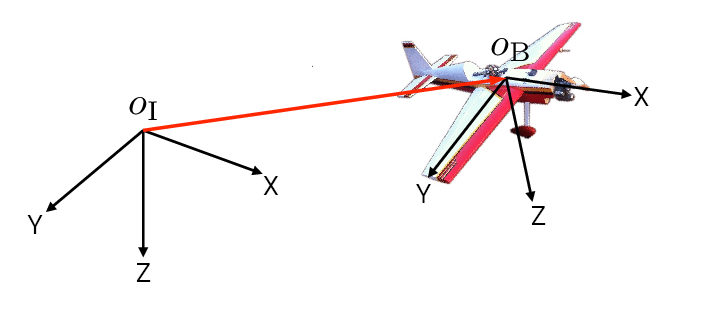
\includegraphics[width=0.7\textwidth]{frames.png}
      	\caption{Definicja układów współrzędnych.}
\end{figure}

Korzystając z przedstawionych układów współrzędnych, można wyrazić poszczególne elementy wektora stanu układu. W tym miejscu należy zaznaczyć, że w nomenklaturze lotniczej przyjmuje się, że symbol $\bm{y}$ oznacza wektor położenia i orientacji BSP wyrażony w globalnym układzie współrzędnych, a symbol $\bm{x}$ oznacza prędkości kątowe i liniowe wyrażone w układzie współrzędnym związanym z BSP. Oznaczenia te kolidują z oznaczeniami wektora stanu i wyjścia z poprzedniego rozdziału. Od tego miejsca wykorzystana zostanie właśnie ta nomenklatura.\\

Położenie i orientacja BSP zdefiniowana jest jako:
\[
	      		 \bm{y} = \begin{bmatrix}x & y &  z & \varphi & \Theta & \Psi  \end{bmatrix}^{T}_{W} \hspace{10pt} \text{lub} \hspace{10pt} \begin{bmatrix}x & y & z & q_0 &  q_x &  q_y & q_z  \end{bmatrix}^{T}_{W},
\]

gdzie $x, y, z$ to położenie, a orientacja BSP wyrażona jest za pomocą trzech kątów lotniczych $\varphi, \Theta,  \Psi$ lub za pomocą kwaternionu orientacji. Wyrażenie orientacji za pomocą kątów lotniczych pozwala w sposób intuicyjny powiązać kąt z orientacją BSP. Pierwszy z kątów $\varphi$ to kąt przechylenia (ang. roll) tj. kąt przechylenia BSP na skrzydło. Dodatni kąt przechylenia to przechylenie samolotu na prawe skrzydło. Drugi z~kątów $\Theta$ to kąt pochylenia (ang. pitch) tj. kąt pochylenia dziobu BSP w górę lub dół. Dodatni kąt pochylenia oznacza dziób zadarty do góry. Ostatni z kątów $\Psi$ opisuje odchylenia (ang. yaw), czyli kąt azymutalny, kierunek kursu. Zerowy kąt odchylenia oznacza skierowanie BSP na północ. Kąt odchylenia może być utożsamiany ze wskazaniem kompasu. Kąty lotnicze zostały dodatkowo przedstawione na rysunku (\ref{RPY}).

\begin{figure}[!h]
   	\centering
      	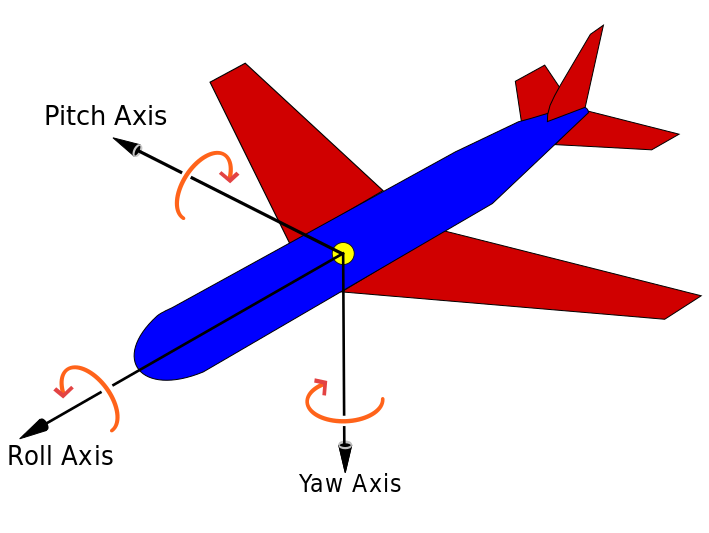
\includegraphics[width=0.5\textwidth]{RPY.png}
      	\caption{Kąty lotnicze.}
      	\label{RPY}
\end{figure}

Oprócz przedstawionych zalet opis orientacji przy pomocy kątów lotniczych ma zasadniczą wadę -- niejednoznaczność. Oznacza to, że ta sama orientacja może zostać wyrażona przy pomocy różnych trójek kątów. Jest to szczególnie ważne dla układu sterowania. Orientacja zadana w kątach lotniczych może różnić się od orientacji aktualnej samolotu jedynie konfiguracją. Tym samym układ będzie wykonywał niepotrzebne zmiany orientacji, które finalnie doprowadziłyby go do tego samego stanu. Bardziej ogólnym sposobem wyrażenia orientacji są kwaterniony. Kwaternion w jednoznaczny sposób definiuje orientację, a także pozwala na obrót pomiędzy układami bez konieczności budowania macierzy rotacji. Można pokazać, że kwaternion odpowiada obrotowi oś-kąt.\\

Kolejnym elementem wektora stanu BSP jest wektor prędkości zdefiniowany następująco:
\[
	\bm{x} = \begin{bmatrix}U & V & W &  P & Q & R  \end{bmatrix}^{T}_{B},
 \]
 
 gdzie U, V i W to prędkości liniowe wyrażone zgodne z wektorami układu ruchomego, a P, Q i R to wektor prędkości kątowej zrzutowany na osie układu ruchomego.\\
 
 Ostatnim elementem wektora stanu BSP jest wektor prędkości kątowych silników:
 \[
	\bm{\omega} = \begin{bmatrix}\omega_1 & \omega_2 & ... &  \omega_{m}  \end{bmatrix}^{T}.
 \]
 Rozmiar wektora $\bm{\omega}$ jest zależny od liczby silników \texttt{m}, w które został wyposażony BSP. W przypadku silników rotorowych odpowiada on bezpośrednio prędkości wału silnika, w przypadku innych silników jest on jedynie miarą rozpędzenia danego silnika.\\
 
Finalnie wszystkie z przedstawionych wektorów ujęte zostają w zbiorczy wektor stanu układu zdefiniowany następująco:
\[
      	\begin{bmatrix} \bm{y}\\ \bm{x} \\  \bm{\omega} \end{bmatrix}.
\]

Po całościowym zdefiniowaniu wektora stanu układu należy poruszyć temat przyjętych jednostek. W projekcie zostało przyjęte założenie o wyrażeniu stanu układu przy pomocy jednostek SI (MKS). Położenie wyrażone jest zatem w metrach, do opisu kątów zastosowane zostały radiany. Prędkości liniowe zostały wyrażone w~metrach na sekundę, a prędkości kątowe w radianach na sekundę.
Co warto zaznaczyć, do wektora stanu mogłyby zostać dodane również inne elementy opisane równaniami różniczkowymi takie jak powierzchnie sterowe bądź inne elementy mechaniczne. W opracowywanym modelu bezwładność tych elementów została jednak pominięta.

\subsubsection{Model matematyczny BSP}

W poprzednim rozdziale zdefiniowany został stan BSP. W tym rozdziale przedstawione zostanie, według jakich praw zmienia się stan układu i co ma na niego wpływ. Zakłada się, że BSP można traktować jako bryłę sztywną, a do zapisania zależności wykorzystane zostaną następujące prawa i twierdzenia:

\begin{enumerate}
\item prędkość jest pochodną położenia,
\item zasada zmienności pędu i krętu, stanowiąca uogólnienie II zasady dynamiki Newtona głosi, że pochodną pędu po czasie jest wypadkowa siła działająca na układ, a pochodną krętu po czasie jest wypadkowy moment działający na układ,
\item silnik można traktować jako człon inercjalny pierwszego rzędu.
\end{enumerate}

Zgodnie z pierwszą zależnością, gdyby położenie i prędkość były wyrażone w tym samym układzie, można by błędnie pomyśleć, że $\bm{\dot{y}} = \bm{x}$. Nie jest to jednak prawdą, gdyż prędkość kątowa nie stanowi bezpośrednio pochodnej kątów lotniczych. Niewątpliwie odpowiednich przekształceń wymaga również wyrażenie pochodnej, gdy orientacja dana jest jako kwaterniony. Wtedy oprócz odpowiedniej transformacji może pojawić się problem nieunormowania kwaternionu tj. niezachowania jednostkowej normy kwaternionu na skutek kumulujących się błędów arytmetyki komputera. Sposobem zapobiegania temu zjawisku jest np. metoda stabilizowania normy kwaternionu. Mając na uwadze wspominane problemy oraz różne układy, w których wyrażone są wektory $\bm{y}$ i $\bm{x}$ można zapisać następującą zależność:
\[
	\bm{\dot{y}} = T(\bm{y}, \bm{x}).
\]

Dla ułatwienia zapisu funkcja T zostanie podzielona na część związaną z położeniem i orientacją. Niech $\bm{r}_W$ oznacza położenie BSP w układzie globalnym, $\bm{v}_B$ jego prędkość wyrażoną w układzie ruchomym, a $\bm{R_B^W}$ to macierz rotacji z układu B do układu W. Wtedy równanie wynikające z funkcji T dla położenia wygląda następująco:
\[
	\bm{\dot{r}}_W = \bm{R_B^W} \bm{v}_B.
\]
W przypadku orientacji $\bm{q}$ funkcja T definiuje jej pochodną w następujący sposób:
\[
	\bm{\dot{q}} = 	\Gamma(P,Q,R) \bm{q} +\left ( 1.0 - \bm{q}^T \bm{q} \right) \cdot \bm{q},
\]
\[
	\Gamma(P,Q,R) = - \frac{1}{2} \cdot \begin{bmatrix}
	0 & P & Q & R \\ -P & 0 & -R & Q \\ -Q & R & 0 & -P \\ -R & -Q & P & 0
	\end{bmatrix},
\]
gdzie pierwszy składnik odpowiada za wpływ prędkości kątowej na zmianę orientacji, a drugi odpowiada za stabilizację normy kwaternionu.\\

Należy sformułować teraz drugą zależność. Pęd bryły sztywnej $\bm{\vec{p}}$ można wyrazić jako:
\[
	\bm{\vec{p}} = m \cdot \bm{\vec{v}},
\]
gdzie $m$ to masa BSP, a $\bm{\vec{v}}$ to wektor jego prędkości liniowych.
Analogicznie kręt (moment pędu) bryły sztywnej $\bm{\vec{L}}$ można wyrazić jako:
\[
	\bm{\vec{L}} = J \cdot \bm{\vec{\omega}},
\]
gdzie $J$ to macierz bezwładności BSP, a $\bm{\vec{\omega}}$ to wektor jego prędkości kątowych. Zgodnie z zasadą zmienności pędu można zapisać następujące zależności:
\[
	\begin{aligned}
	\frac{d\bm{\vec{p}}}{dt} & = \bm{\vec{F}},\\
	\frac{d\bm{\vec{L}}}{dt} & = \bm{\vec{\tau}},
	\end{aligned}
\]
gdzie $\bm{\vec{F}}$ to wypadkowa siła przyłożona do BSP, a $\bm{\vec{\tau}}$ to wypadkowy moment siły działający na BSP. Korzystając z własności rachunku macierzowego, powyższe zależności można połączyć, uzyskując tym samym zależność:
\[
              \begin{bmatrix}\frac{d\bm{\vec{p}}}{dt}\\ \frac{d\bm{\vec{L}}}{dt} \end{bmatrix} = \begin{bmatrix}\bm{\vec{F}}\\ \bm{\vec{\tau}} \end{bmatrix} = \bm{\vec{f}},
\]
gdzie $\bm{\vec{f}}$ to uogólnione oddziaływanie na układ. Na koniec poprzez policzenie odpowiednich pochodnych (pamiętając o regule pochodnej iloczynu) możliwe jest uproszczenie zapisu do postaci:

\[
	\bm{M} \bm{\dot{x}} +  \bm{\Omega} \left( \bm{x} \right) \bm{M} \bm{x} = \bm{f},
\]
\[
	\bm{\Omega} = \begin{bmatrix}
	0 & -R & Q & 0 & 0 & 0 \\
	R & 0 & -P & 0 & 0 & 0 \\
	-Q & R & 0 & 0 & 0 & 0 \\
	0 & -W & V & 0 & -R & Q \\
	W & 0 & -U & R & 0 & -P \\
	-V & U & 0 & -Q & P & 0 
	\end{bmatrix}
	\vspace{10pt}
	\bm{M} = \begin{bmatrix}
	m\cdot \bm{ I_{3x3}} & \bm{0_{3x3}} \\ \bm{0_{3x3}} & \bm{J}
	\end{bmatrix},
\]
gdzie $\bm{M}$ jest macierzą masową powstałą przez połączenie masy i macierzy bezwładności, a $\bm{\Omega}$ to tzw. macierz żyroskopowa.\\

Ostatnia z przedstawionych na początku rozdziału zależności dotyczy zachowania silnika. Przyjętym modelem dla silnika elektrycznego jest człon inercyjny pierwszego rzędu. W takim modelu wartość przyśpieszenia kątowego jest zależna od różnicy pomiędzy wartością zadaną a aktualną. W teorii sterowania różnicę tą nazywa się uchybem. Dodatkowo w modelu występuje współczynnik skalujący nazywany stałą czasową T. Układ równań różniczkowych opisujących zachowanie silnika wyraża się następująco:
 \[
	T \frac{d\omega}{dt} + \omega = \omega_{ZADANA},
\]
gdzie $\omega_{ZADANA}$ to prędkości kątowe zadane przez układ sterowania. 

\begin{figure}[!h]
   	\centering
      	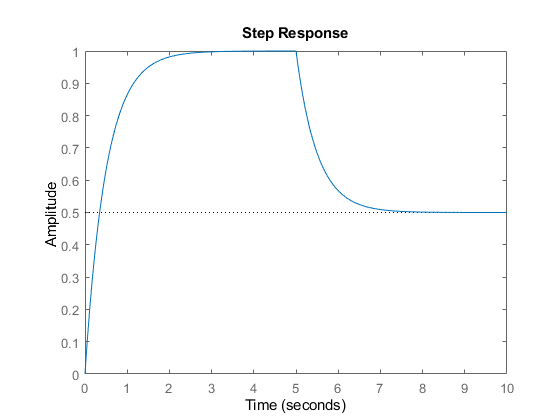
\includegraphics[width=0.6\textwidth]{step.png}
      	\caption{Odpowiedź układu inercyjnego pierwszego rzędu.}
      	\label{rotor_step}
\end{figure}

Dla zilustrowania zachowania silnika na rysunku (\ref{rotor_step}) przedstawiono wykres prędkości kątowej silnika w funkcji czasu. W chwili początkowej silnikowi zadana została znormalizowana wartość prędkości wynosząca 1. W 5 sekundzie ruchu wartość zadana została zmieniona na 0.5. Należy zwrócić uwagę, że stała T ma dokładną interpretację fizyczną i jest to czas, po którym spoczywający układ osiągnie 63.5\% wartości zadanej. Przy okazji warto wspomnieć, że $\omega_{ZADANA}$ stanowi zasadniczą cześć sterowania BSP.

\subsubsection{Siły i momenty działające na BSP}

Przedstawiony w poprzednim rozdziale model przyjmował, że na układ działa uogólnione oddziaływanie $\bm{\vec{f}}$. W tym rozdziale omówione zostaną poszczególne składowe, które sumują się na to oddziaływanie.\\

Wszystkie oddziaływania powinny być wyrażone w układzie ruchomym związanym z BSP. W ramach tego projektu przyjęte zostało, że na BSP wpływają następujące oddziaływania:
\begin{itemize}
  \item {
    siła grawitacji  $\bm{f_G}$,
  }
  \item{   
    ciąg silników i moment oporowy  $\bm{f_R}$,
   }
    \item{   
    ciąg silników marszowych  $\bm{f_J}$,
   }
    \item{   
    oddziaływanie aerodynamiczne $\bm{f_A}$,
   }
    \item{   
   siły zewnętrzne $\bm{f_{OUT}}$.
   }
\end{itemize}

\textbf{Siła grawitacji  $\bm{f_G}$} to siła zależna od masy BSP przyłożona w jego środku masy, wyrażona we właściwym układzie współrzędnych.

\[
	 \bm{f_G} = \begin{bmatrix} \bm{R_W^B}\begin{bmatrix}0 & 0 & m \cdot g\end{bmatrix}^T  \\ \bm{0_{3x1}}  \end{bmatrix},
\]
gdzie $\bm{R_B^W}$ to macierz rotacji z układu W do układu B.\\

\textbf{Ciąg silników i moment oporowy  $\bm{f_R}$} to siła i moment generowany przez obracający się wirnik. Wartość siły i momentu $F$ i $M$ zależy od prędkości kątowej wirnika $\omega$, promienia wirnika $R$, powierzchni tworzonej przez wirnik $S$, gęstości powietrza $\rho$ oraz współczynników $k_F$ oraz $k_M$:
\[
	\begin{aligned}
	F_R & = k_F \rho S R^2 \omega^2,\\
	M_R & = k_M \rho S R^3 \omega^2.
	\end{aligned}
\]

Wirnik jest zamontowany w pewnym konkretnym miejscu BSP, określonym przez wektor $\bm{\vec{r_R}}$ i~skierowany według wersora $\bm{\vec{a_R}}$. Oba wektory wyrażone są w układzie związanym z~BSP. Całkowite oddziaływanie generowane przez wirnik wynosi wtedy:
\[
	\bm{f_R} =  \begin{bmatrix} F_R \cdot  \bm{\vec{a_R}} \\   \pm M_R \cdot \bm{\vec{a_R}} \pm  \bm{\vec{r_R}} \times \left( F_R \cdot  \bm{\vec{a_R}} \right) \end{bmatrix}.
\]
Niejednoznaczność dotycząca kierunku działania momentu wynika z kierunku obracania się wirnika. Jeśli siła i kierunek obrotu są zgodne z zasadą prawej ręki, to przy momencie znajduje się plus. W przeciwnym przypadku -- minus.\\

\textbf{Ciąg silników marszowych $\bm{f_R}$} to siła generowana przez silnik odrzutowy montowany najczęściej w rakietach. W przypadku tego silnika generowana jest jedynie siła zgodna z kierunkiem działania $\bm{\vec{a_J}}$. W projekcie ciąg takiego silnika $F_J$ jest funkcją czasu i został zdefiniowany jako tablica par czas-wartość. W~punktach pośrednich wartość jest interpolowana przy pomocy funkcji liniowej. Mając wartość ciągu w danej chwili czasu i miejsce zamontowania silnika $\bm{\vec{r_J}}$ można wyznaczyć oddziaływanie generowane przez silnik:
\[
	\bm{f_J} =  \begin{bmatrix} F_J \cdot  \bm{\vec{a_J}} \\  \bm{\vec{r_J}} \times \left( F_J \cdot  \bm{\vec{a_J}} \right) \end{bmatrix}.
\]

\textbf{Oddziaływanie aerodynamiczne $\bm{f_A}$} to oddziaływanie wynikające z wpływu powietrza, w którym porusza się BSP. Mogą one mieć charakter bierny, tak jak siła oporu powietrza, lub być celowo wykorzystywane do lotu, jak ma to miejsce w~przypadku siły nośnej i oddziaływań generowanych przez powierzchnie sterowe. Oddziaływanie aerodynamiczne można zamodelować jako \cite{solar_plane}:
\[
	\bm{f_A} = \frac{1}{2}\rho V_{T}^2  \bm{S} \bm{C}\left(\alpha, \beta, \bm{x}, \bm{\delta}, ... \right),
\]
gdzie $\rho$ to gęstość powietrza, $V_T$ to moduł prędkości BSP względem powietrza, $S$ to macierz diagonalna zawierająca na diagonali wymiary charakterystyczne BSP, a $C$ to wektor współczynników aerodynamicznych wynikający z kształtu i budowy BSP. Iloczyn $\frac{1}{2}\rho V_{T}^2$ jest tzw. ciśnieniem dynamicznym i jest on ściśle związany z~zagadnieniem prędkości indukowanej. Jeśli wektor prędkości powietrza w układzie związanym z BSP wyrazimy jako $ \begin{bmatrix} U_W & V_W & W_W\end{bmatrix}^T$ to $V_T$ wynosi:
\[
	V_T = \sqrt{(U-U_W)^2 + (V-V_W)^2 + (V-V_W)^2},
\]
natomiast kąt natarcia $\alpha$ oraz kąt ślizgu $\beta$ wynoszą odpowiednio:
\[
	\alpha = atan2 \left( W - W_W, U - U_W \right),
\]
\[
	\beta = asin \left( \frac{V-V_W}{V_T} \right).
\]

Do zdefiniowania pozostaje wektor współczynników aerodynamicznych $C$. W ogólności wartość współczynników zależy od niemal wszystkich aspektów i parametrów BSP. Często do jego przestawienia wykorzystuje się wielowymiarowe mapy generowane w specjalistycznych programach. Dla uogólnienia często stosowanym rozwiązaniem jest linearyzacja współczynników wokół pewnego punktu równowagi:
\[
\bm{C} \approx \bm{C0} + \frac{d\bm{C}}{d\alpha}\alpha + \frac{d\bm{C}}{d\beta}\beta + \frac{d\bm{C}}{d\bm{x}}\bm{x} + \frac{d\bm{C}}{d\bm{\delta}}\bm{\delta}.
\]
W przedstawionym wyżej przypadku linearyzacja odbywa się wokół punktu oznaczającego lot z zerowym kątem natarcia i ślizgu, zerowymi prędkościami oraz neutralnym położeniem powierzchni sterowych i jest jednoznacznie definiowana przez macierze pierwszych pochodnych i wartość zerową. Dokładniejszy model można uzyskać na drodze rozwinięcia szeregu Maclaurina do kolejnych pochodnych.\\

Przedstawiony model pozwala na uzyskanie zadowalających wyników jedynie w otoczeniu punktu równowagi. Dla uzyskania dokładniejszych odpowiedzi, a także, aby uzyskać pożądany efekt przeciągnięcia, należy określić współczynniki aerodynamiczne dla dużych kątów natarcia. Jednym ze sposobów na zapewnienie takiego zachowania BSP jest przyjęci, że poza ograniczonym zakresem kąta natarcia współczynniki aerodynamiczne związane z oporem powietrza i siłą nośną są nadpisywane przez wartości $C_D = 1 - cos(2 \cdot \alpha)$ oraz $C_L = sin(2 \cdot \alpha)$. Interpretacja tego podstawienia sprowadza się do założenia, że dla dużych wartości kąta natarcia, BSP należy traktować jako płaską powierzchnię o rozmiarze płata.\\


\textbf{Siły zewnętrzne $\bm{f_{OUT}}$} to pozostałe siły działające na BSP. Mogą to być dowolne siły i momenty zredukowane do oddziaływania przyłożonego w środku masy BSP. W projekcie oddziaływaniami zewnętrznymi działającymi na BSP są siła i moment pochodzące od liny łączącej BSP z ładunkiem.

\subsubsection{Warunki atmosferyczne. Model atmosfery ISA}

W przedstawionym modelu dynamiki pojawiają się odniesienia do warunków atmosferycznych, w których wykonywany jest lot. Siła i moment generowany przez silniki zależą m.in. od gęstości powietrza. Oddziaływania aerodynamiczne zależą m.in. od prędkości wiatru i gęstości powietrza. Z tego względu kolejną częścią modelu jest zaplanowanie, w jaki sposób zdefiniować potrzebne warunki atmosferyczne.\\

Ruch powietrza, zwany powszechnie wiatrem można zdefiniować jako wektorowe pole prędkości. Oznacza to wyrażenie każdej z trzech składowych wektora prędkości jako funkcji położenia. Jeśli pożądane jest, aby wiatr zmieniał się w czasie symulacji, wspomniane funkcje należy uzależnić również od czasu. W ogólności wiatr nie ma charakteru stałego i ze względu na występowanie przeszkód występują w nim lokalne zaburzenia pola prędkości zwane również turbulencjami. Jeśli jednak ograniczyć się do stacjonarnego modelu liniowego to pole prędkości można w prosty sposób przedstawić jako:

\[
	\begin{bmatrix} U_W \\ V_W \\ W_W\end{bmatrix} = \bm{A} \begin{bmatrix} x \\ y \\ z\end{bmatrix}  + \bm{b} + \bm{\epsilon},
\]
gdzie $\bm{A}$ i $\bm{b}$ to macierz i wektor definiujące pole wektorowe, a $\bm{\epsilon}$ to wektor modelujący turbulencje. Należy nadmienić, że istnieją również bardziej wyrafinowane modele ruchu powietrza, uwzględniające spowolnienie strugi w warstwie przypowierzchniowej, jak np. the U.S. Naval Research Laboratory Horizontal Wind Model (HWM™).

W przypadku skalarnych parametrów atmosferycznych takich jak temperatura, ciśnienie i gęstość powietrza, ich zmiany zachodzą znaczenie wolniej. W danym punkcie przestrzeni zmiana tych parametrów na przestrzeni kilku minut, a nawet godzin jest na ogół bardzo niewielka. Inaczej wygląda to w przypadku zmian położenia -- o~tej samej porze w różnych punktach przestrzeni warunki atmosferyczne mogą różnić się znacznie. W szczególności, duży wpływ ma zmiana wysokości. Z elementarnej wiedzy z przyrody znana jest ciekawostka, że zmianie wysokości o 1000m towarzyszy spadek temperatury o ok. 6$^{\circ}C$. Na potrzeby symulacji potrzebny jest jednak bardziej sformalizowany model. Powszechnie wykorzystywanym jest model standardowy atmosfery ISA (ang. International Standard Atmosphere). Przy pomocy tego modelu można oszacować temperaturę, ciśnienie i gęstość powietrza w zależności od wysokości nad przyjętym punktem odniesienia $h$. W obliczaniach potrzebna jest również temperatura $T_0$ i ciśnienie $p_0$ w punkcie odniesienia. Według modelu, w warstwie troposfery temperaturę $T(h)$, ciśnienie $p(h)$ i gęstość $\rho(h)$ można obliczyć za pomocą wzorów:
\[
	\begin{aligned}
	T(h) & = T_0 - h \cdot 0.0065 \frac{^\circ C}{m},\\
	p(h) & = p_0 \cdot \left(1.0 - 0.0065 \frac{^\circ C}{m} \cdot \frac{h}{T_0} \right)^{\frac{g}{R \cdot  0.0065 \frac{^\circ C}{m}}},\\
	\rho(h) &  = \frac{p(h)}{T(h) \cdot R},
	\end{aligned}
\]
gdzie $g$ to przyśpieszenie grawitacyjne (9.8067 $\frac{m}{s^2}$), a $R$ to indywidualna stała gazowa powietrza (287.052874  $\frac{J}{kg \cdot K}$). Zakres stosowalności powyższych wzorów obejmuje wysokości do ok. 11000 m.n.p.m.

\subsubsection{Kolizje}

W trakcie lotu BSP może zderzyć się z otoczeniem, innym BSP lub wystrzelonym obiektem. W rzeczywistości takie zderzenie powoduje odbicie, nierzadko połączone ze zniszczeniem statku. Zakres pojęcia kolizji można również uogólnić, uznając, że każde lądowanie jest swoistą kolizją BSP z otoczeniem. Z tego powodu, dla zachowania odpowiedniego realizmu w symulacji, istotne jest wykrywanie kolizji w trakcie lotu i skuteczna reakcja na nie.\\

Najprostszym sposobem na wykrycie kolizji pomiędzy dwoma obiektami jest obliczenie odległości pomiędzy ich środkami masy. Taka metoda pomija kształt geometryczny obiektów, zakładając, że oba obiekty mają kształt kuli. Odległość, poniżej której powinno być zarejestrowane zderzenie, jest sumą promieni kul, którymi przybliżamy potencjalnie kolidujące obiekty. Metoda ta nie pozwala określić, która część obiektu uległa kolizji, ale dzięki swojej prostocie jest niezwykle wydajna. Jej zastosowanie ogranicza się do przypadków, w których obiekty po kolizji należy uznać za zniszczone, np. trafienie BSP pociskiem powoduje jego zniszczenie.\\

W grafice komputerowej do przechowywania geometrii obiektów służą pliki zawierające model 3D. W przypadku najprostszego z nich -- pliku OBJ -- model przechowywany jest jako lista wierzchołkami oraz lista wielokątów opartach na tych wierzchołkach. Jako że przy pomocy prostego algorytmu można rozłożyć dowolny wielokąt na trójkąty bez straty ogólności, można uznać, że geometria obiektu reprezentowana jest przez siatkę trójkątów.\\

Kolejna metoda wykrywania kolizji polega sprawdzeniu, czy zaistniała kolizja pomiędzy obiektem przybliżonym kulą a obiektem o określonej geometrii. Znana jest: pozycja i prędkość pierwszego obiektu oraz promień kuli przybliżającej jej kształt, a~także pozycja drugiego obiektu danego siatką trójkątów. Metoda zakład, że obiekt siatkowy spoczywa, przez co idealnie nadaje się do sprawdzania kolizji z niezmiennym otoczeniem. Sprawdzenie, czy pomiędzy obiektami zaszła kolizja, polega na sprawdzeniu, czy środek pierwszego obiektu znajduje się dostatecznie blisko któregokolwiek trójkąta z siatki. W tym celu wykorzystuje się zrzut prostokątny na powierzchnie zawierającą trójkąt. Efektem obliczeń jest odległość punktu od płaszczyzny oraz jego współrzędne barycentryczne. Jeśli moduł odległości jest mniejszy od promienia kuli i rzut należy do trójkąta, rejestrowana jest kolizja w rzutowanym punkcie. Ze względu na ograniczoną częstotliwość sprawdzania kolizji, należy przewidzieć również, gdzie znajdzie się obiekt po okresie sprawdzania i, czy w tym przedziale czasu nie zajdzie kolizja. Wykorzystując prędkość i okres, można przy pomocy jawnego algorytmu Eulera wyznaczyć estymowane położenie obiektu.\\

Algorytm obliczenia rzutu prostokątnego wygląda następująco: Niech $A$,$B$ i $C$ będą wektorami określającymi pozycję trójkąta w przestrzeni, a $P$ będzie rzutowanym punktem. Wtedy:
\[
	\begin{bmatrix}
	a \\ b \\ h
	\end{bmatrix}
	=
	\begin{bmatrix}
	B - A & C - A & (B - A) \times (C - A)
	\end{bmatrix}^{-1} \left( P - A \right),
\]
gdzie $a$ i $b$ to współrzędne barycentryczne rzutu w trójkącie $ABC$, a $h$ to odległość punktu $P$ od płaszczyzny trójkąta $ABC$. Dodatkowo, jeśli spełnione jest, że:
\[
a \geq 0 \land b \geq 0 \land a + b \leq 1,
\]
to rzut należy do trójkąta $ABC$.\\

Ostatnia z metod wykrywania kolizji pozwala na wykrycie kolizji pomiędzy dwoma obiektami danymi siatką trójkątów. Pozostaje w mocy założenie, że jeden z obiektów spoczywa, oraz znane jest położenie i prędkości drugiego z obiektów. W tej metodzie drugi z~obiektów traktowany jest jako chmura punktów. Z posiadanych danych możliwe do wyznaczenia jest położenie $P$ i prędkość $v_P$ każdego z wierzchołków. Metoda polega na sprawdzeniu, czy w nadchodzącym okresie sprawdzenia $T$ promień zdefiniowany przez punkt i prędkość przebije dowolny z trójkątów z~siatki drugiego obiektu. Do określenia punktu przebicia wykorzystać można algorytm Möllera–Trumbore'a \cite{ray_intersaction}. Rezultatem działania algorytmu jest określenie we współrzędnych barycentrycznych, gdzie znajduje się punkt przebicia oraz jaka jest odległość pomiędzy punktem $P$, a~punktem przebicia $t$. Jeśli $t > 0 \land t < T\cdot |v_P|$. rejestrowana jest kolizja. Oczywistą wadą tego algorytmu jest pominięcie kolizji, które miały miejsce wewnątrz trójkąta pierwszego z obiektów. Przekłada się to np. na niewykrywanie kolizji BSP z wąskimi liniami energetycznymi. Mając jednak na uwadze wady tej metody, można dobrać na tyle gęstą siatkę obiektu, aby wykryć zdecydowaną większość kolizji.\\


Kolejnym etapem po wykryciu kolizji jest właściwe zamodelowanie reakcji BSP. Podtrzymane zostaje założenie, że BSP jest bryłą sztywną.  Dane są: położenie BSP $\bm{\vec{r}}$, jego prędkość liniowa $\bm{\vec{v}}$ oraz kątowa $\bm{\vec{\omega}}$, a także macierz masowa $\bm{M}$. Wykryta została kolizja BSP z nieruchomą ścianą o wektorze normalnym $\bm{\vec{n}}$ w punkcie $\bm{\vec{r_P}}$. Jedną z~metod modelowania takiej kolizji jest przyłożenie do BSP siły zgodnej z wektorem normalnym w punkcie kolizji. Problemem tej metody jest to, że kolizję trwają bardzo krótko. Ze względu na znacznie większy krok symulacji doprowadziłoby to do powstawania znacznych błędów. Znacznie dokładniejsze wyniki dostarcza metoda kolizji impulsowych \cite{impulse_collision}. Ideą tej metody jest założenie, że czas trwania kolizji jest pomijanie mały, a całą kolizję należy traktować jako impuls. W związku z~tym wynikiem obliczeń jest stan, a konkretnie prędkość BSP po kolizji, która ulega skokowej zmianie. Model kolizji impulsowych pozwala określić stan po zderzeniu z~uwzględnieniem siły normalnej do powierzchni oraz tarcia stycznego. Ponadto poprzez zmianę jednego parametru, nazywanego COR (ang. coefficient of restitution) możliwa jest płynna regulacja pomiędzy zderzeniem plastycznym (COR = 0) a sprężystym (COR = 1). Co ciekawe ten sam model może być wykorzystany do zderzeń, w których generowana jest energia (COR > 1) oraz dla zderzeń z penetracją ( COR < 0).\\

W pierwszym etapie metody konieczne jest obliczenie wartości impulsu siły. Fizycznie impuls siły $\bm{\vec{j}}$ jest całką z siły reakcji ściany w trakcie trwania kolizji:
\[
	 \bm{\vec{j}} = \int_{t_0}^{t_1} \bm{\vec{F}} dt.
\]

W metodzie oddzielnie rozpatruje się impuls związany z reakcją normalną\\ $j_r \left( \bm{M}, \bm{\vec{v}}, ...  , COR \right)$ i reakcją styczną $j_f \left( \bm{M}, \bm{\vec{v}}, ...  , \mu_s, \mu_d \right)$. Po obliczeniu wartości impulsów prędkości po kolizji wynoszą 
\[
	\begin{aligned}
	\bm{\vec{v}}_{po} & = \bm{\vec{v}}_{przed} - \frac{j_r}{m} \bm{\vec{n}} - \frac{j_f}{m} \bm{\vec{t}},  \\
	\bm{\vec{\omega}}_{po} & = \bm{\vec{\omega}}_{przed} - j_r \cdot \bm{J}^{-1} \left(  \bm{\vec{r_P}} \times \bm{\vec{n}} \right) - j_r \cdot \bm{J}^{-1} \left(  \bm{\vec{r_P}} \times \bm{\vec{t}} \right),
	\end{aligned}
\]
gdzie: $\bm{\vec{t}}$ to wektor styczny do powierzchni i przeciwny do rzutu wektora prędkości na powierzchnię.

\subsubsection{Odrzut}

Kiedy z BSP wystrzelony zostaje pocisk o niezerowej prędkości względnej, statek doznaje zjawiska odrzutu. Odrzut to skokowa zmiana prędkości BSP na skutek oddzielania się części jego masy (w postaci pocisku) będąca następstwem zasady zachowania pędu. Głosi ona, że w układzie izolowanym, pęd i kręt pozostają stałe. W przypadku wystrzelenia pocisku zasadę tą można sformułować jako:
\[
	\begin{bmatrix}
	\vec{\bm{p}}_{przed}\\
	\vec{\bm{L}}_{przed}
	\end{bmatrix}
	=
	\begin{bmatrix}
	\vec{\bm{p}}_{po}\\
	\vec{\bm{L}}_{po}
	\end{bmatrix}
	+	
	\begin{bmatrix}
	\vec{\bm{p}}_{pocisku}\\
	\vec{\bm{L}}_{pocisku}
	\end{bmatrix}.	
\]
Jeśli pocisk potraktowany zostanie jako punkt materialny o masie $m_{pocisku}$:
\[
	\bm{M}_{przed}
	\begin{bmatrix}
	\vec{\bm{v}}_{przed}\\
	\vec{\bm{\omega}}_{przed}
	\end{bmatrix}
	=
	\bm{M}_{po}
	\begin{bmatrix}
	\vec{\bm{v}}_{po}\\
	\vec{\bm{\omega}}_{po}
	\end{bmatrix}
	+
	m_{pocisku}
	\begin{bmatrix}
	\vec{\bm{v}}_{pocisku}\\
	\vec{\bm{r}}_{pocisku} \times  \vec{\bm{v}}_{pocisku}
	\end{bmatrix},
\]
gdzie $\vec{\bm{r}}_{pocisku}$ to wektor łączący punkt wystrzału pocisku, ze środkiem ciężkości BSP. Należy również określić układ współrzędnych, w którym wyrażone są wektory prędkości. Jako że macierz bezwładności $J$ została określona w układzie związanym BSP, to właśnie w tym układzie należy przeprowadzić powyższe obliczenia. Gdyby zaistniała potrzeba wykonywania obliczeń w układzie globalnym, do przeliczenia macierzy bezwładności między układami należy wykorzystać twierdzenie Steinera:
\[
	J_W = R_B^W J_B (R_B^W)^T - m \tilde{\vec{\bm{r}}} \tilde{\vec{\bm{r}}},
\]
gdzie $ \tilde{\vec{\bm{r}}}$ to macierz stowarzyszona do wektora $\vec{\bm{r}}$ wyrażającego położenie BSP w układzie globalnym.\\

Skutkiem wystrzału jest zmiana masy i momentu bezwładności BSP. Znając masę pocisku i położenie pocisku możliwe jest obliczenie masy i momentu bezwładności BSP po wystrzale, korzystając ponownie z tw. Steinera:
\[
	\begin{aligned}
	m_{po} & = m_{przed} - m_{pocisku},\\
	J_{po} & = J_{przed}  - ( - m \tilde{\vec{\bm{r}}}_{pocisku} \tilde{\vec{\bm{r}}}_{pocisku} ). 
	\end{aligned}
\]

Dla kompletności poniższe wzory pozwalają na obliczenie położenia i prędkości pocisku w układzie globalnym w chwili wystrzału:
\[
	\begin{aligned}
	\vec{\bm{r}}_{pocisku}^W & = \vec{\bm{r}} + R_B^W \vec{\bm{r}}_{pocisku},\\
	\vec{\bm{v}}_{pocisku}^W & =  R_B^W \left( \vec{\bm{v}}_{pocisku} + \vec{\bm{\omega}}_{przed} \times \vec{\bm{r}}_{pocisku} \right).\\
	\end{aligned}
\]



\subsubsection{Przenoszenie ładunku}

Głównym zastosowaniem niektórych BSP jest przenoszenie ładunku. Ładunek może być zlokalizowany wewnątrz statku, pozostając z nim sztywno połączonym, lub znajdować się na zewnątrz BSP. Najczęściej do połączenia ładunku ze statkiem stosuje się różnego rodzaju liny lub sztywne cięgna. Takie połączenie zostaje rozpięte pomiędzy wybranym punktem BSP a wybranym punktem ładunku. Jeśli ładunek traktowany jest jako punkt masowy, to wybór mocowania ładunku staje się jednoznaczny.\\

Linę rozpiętą między dwoma punktami można zamodelować jako równoległe połączenia sprężyny o stałej sprężystości $k$ i tłumika wiskotycznego o współczynniku tłumienia wynoszącym $b$. Lina posiada pewną spoczynkową długość $l_0$. Położenia punktów dane są we wspólnym układzie współrzędnych jako $\vec{\bm{r}}_{A}$ i $\vec{\bm{r}}_{B}$, a ich prędkości oznaczone zostały jako $\vec{\bm{v}}_{A}$ i $\vec{\bm{v}}_{B}$. Jeśli odległość pomiędzy punktami jest mniejsza niż $l_0$:
\[
	| \vec{\bm{r}}_{A} - \vec{\bm{r}}_{B} | < l_0.
\]
To lina pozostaje nienapięta i wypadkowa siła w punktach przyłączenia wynosi zero. Jeśli natomiast punkty oddalą się od siebie o odległość większą niż $l_0$ to w punktach mocowania pojawi się siła wynikająca z rozciągnięcia liny. Oznaczmy jako $\vec{\bm{d}}$ wektor wskazujący kierunek i długość liny:
\[
	\vec{\bm{d}} =  \vec{\bm{r}}_{B} - \vec{\bm{r}}_{A}.
\]
Siła reakcji liny działająca w punkcie A wynosi:
\[
	\vec{\bm{F}}_{A} =\left(  k \cdot \left( |\vec{\bm{d}}| - l_0 \right) + b \cdot \left( \vec{\bm{v}}_{B}  \circ \frac{\vec{\bm{d}}}{|\vec{\bm{d}}|} - \vec{\bm{v}}_{A} \circ \frac{\vec{\bm{d}}}{|\vec{\bm{d}}|} \right) \right)  \cdot \frac{\vec{\bm{d}}}{|\vec{\bm{d}}|}.
\]
Z III zasady dynamiki Newtona wynika natomiast, że siła działająca w drugim z~punktów $\vec{\bm{F}}_{B} = - \vec{\bm{F}}_{A}$. Należy jeszcze przypomnieć, że choć sama lina nie generuje w punkcie przyłożenia momentu (jej mocowanie modelowane jest parą sferyczną) to ze względu na punkt mocowania w BSP może ona generować niezerowy moment wypadkowy. Niech $\vec{\bm{r}}_{H}$ będzie wektorem łączącym środek ciężkości BSP z punktem mocowania liny, a $\vec{\bm{F}}_{H}$ siłą przetransformowaną do układu związanego z BSP. Wtedy:
\[
	\bm{f_{OUT}} = \begin{bmatrix} \vec{\bm{F}}_{H} \\ \vec{\bm{r}}_{H} \times \vec{\bm{F}}_{H} \end{bmatrix}.
\]


\subsection{Sterowanie BSP}

Sterowanie statkiem powietrznym to proces kontroli ruchu, trajektorii i orientacji statku. Jest to zatem sposób na wymuszenie na BSP określonego zachowania. Historycznie sterowanie statkami powietrznymi (wtedy tylko płatowcami) sprowadzało się do wychylenia odpowiednich powierzchni sterowych, które przy pomocy cięgien były spięte ze sterem i pedałami. Z biegiem lat pojawiły się bardziej zaawansowane rozwiązania, co w rezultacie niemal całkowicie uzależniło sterowanie od wbudowanych systemów sterowania. Wiele konstrukcji byłoby praktycznie niemożliwych do pilotowania, gdyby nie zostały wyposażone w odpowiedni układ sterowania.\\


Celem tego rozdziału jest przedstawienie podstawowych pojęć związanych ze sterowaniem. W rozdziale zostaną wprowadzone podstawy teorii sterowania, a także zaprezentowane zostanie wykorzystanie tej wiedzy w kontekście sterowania statkiem powietrznym. Omówione zostaną również podstawy nawigacji, która stanowi nieodłączny element procesu sterowania.

\subsubsection{Regulacja i sterowanie}

Przed rozpoczęciem projektowania systemu sterowania BSP należy przybliżyć podstawy wynikające z teorii sterowania. Z definicji, sterowanie to proces mający na celu takie oddziaływanie na sterowany obiekt, aby ten zachowywał się w określony, zaplanowany sposób. W sterowaniu głównym zadaniem jest taki dobór sygnałów sterujących, aby spowodować zmianę aktualnego stanu obiektu na oczekiwany, przy jednoczesnym spełnieniu istniejących ograniczeń. Regulacja natomiast to proces mający na celu odtworzenie i utrzymanie zadanej wartości, danej przez pewien wzorzec.\\

Zasadniczym podziałem systemów sterowania jest podział na układy otwarte i układy zamknięte. Układy sterowania otwartego to układy, gdzie system sterowania nie posiada informacji zwrotnej ze sterowanego obiektu. Przykładem takiego sterowania jest układ czasowy w tosterze. Jego zdaniem jest jedynie ogrzewanie tosta przez określony czas. Układ nie wie nic o stanie wypieczenia, a tym samym nie potrafi dopasować się do użytego rodzaju pieczywa. Przeciwieństwem do układów otwartych są układy z zamkniętą pętlą sterowania nazywane również układami ze sprzężeniem zwrotnym. W układach tych na bieżąco dokonuje się pomiaru wartości sterowanej i~porównuje się go z wartością zadaną. Różnice pomiędzy wartością zadana a aktualną nazywa się uchybem. W układach zamkniętych system sterowania nie operuje na pojęciach bezwzględnych jak np. stopień wypieczenia, a na pojęciach względnych: za mało, za dużo. Układ, którego zadaniem będzie utrzymanie wartości wejściowej, nazywany jest układem regulacji.\\

Na rysunku (\ref{reg}) przestawiono klasyczny układ regulacji.  Wejście do układu stanowi sygnał zadany $w$. Następnie sygnał ten porównywany jest z wartością mierzoną przez układ pomiarowy, w efekcie czego uzyskiwany jest uchyb $e$. Uchyb trafia na regulator, którego celem jest wykorzystanie urządzeń wykonawczych do takiego sterowania obiektem, aby jego sygnał wyjściowy $x$ jak najlepiej odpowiadał wartości zadanej. W praktyce każdy z tych sygnałów obarczony jest błędem, co należy przewidzieć, projektując regulator. Podsumowując, celem zadania regulacji jest dla danego obiektu wyposażonego w układy wykonawcze tak dobrać regulator i układ pomiarowy, aby zapewnić jak najlepsze śledzenie wartości zadanej, według przyjętego kryterium.

\begin{figure}[!h]
   	\centering
      	\includegraphics[width=0.8\textwidth]{uk\_reg.jpg}
      	\caption{Klasyczny układ regulacji.}
      	\label{reg}
\end{figure}

\subsubsection{System sterowania BSP}
System sterowania BSP jest układem regulacji, w którym wartością regulowaną są parametry lotu. Do najważniejszych parametrów lotu zaliczyć można prędkość i~kierunek lotu, wysokość, orientację BSP oraz jego położenie w przestrzeni. Obiektem sterowanym jest BSP. Układy wykonawcze stanowią silniki i powierzchnie sterowe. Układ pomiarowy stanowi układ nawigacji, zamontowany na BSP. Wartość zadana jest wprowadzana przez operatora.

 Ze względu na poziom automatyzacji dokonuje się podziału systemów sterowania na trzy następujące po sobie segmenty:
\begin{itemize}
\item system stablizacji,
\item autopilot,
\item system zarządzania lotem (generator trajektorii).
\end{itemize}
System stabilizacji to system zapewniający stabilny lot ustalony. Zadaniem tego systemu jest gaszenie prędkości kątowych i utrzymanie stabilnego lotu bez aktywnej zmiany kierunku i prędkości lotu. W samolotach statycznych aerodynamicznie obecność tego systemu nie jest wymagana, gdyż stabilność wynika bezpośrednio z~konstrukcji samolotu.\\

Autopilot to system zapewniający regulację pojedynczego parametru lotu. Może dbać o utrzymanie prędkości, utrzymanie kierunku lotu lub wysokości. Autopilot odciąża pilota z obowiązku kontrolowania poszczególnych elementów stanu BSP.\\

System zarządzania lotem to układ stanowiący ostatni etap w BSP o dużym stopniu autonomii. System operuje na pojęciach punktu i orientacji zadanej. Automatycznie dobiera sterowanie, pozwalające na osiągniecie celu. W przypadku płatowców układ sterowania lotem dodatkowo wytycza trajektorię, która umożliwi osiągnięcie celu.\\

Na rysunku (\ref{control_3_stage}) przedstawiono układ sterowania BSP z uwzględnieniem pilota/operatora. Segmenty zostały przedstawione w sposób ideowy jako układy MIMO (ang. multiple input multiple output). Wewnątrz, każdy z tych segmentów składa się z~wielu regulatorów realizujących zadanie regulacji pojedynczych, bardziej elementarnych wartości jak np. prędkości przechylania lub kąta odchylenia. Rysunek (\ref{pid_ladder}) prezentuje pełny układ sterowania wielowirnikowcem zbudowany z regulatorów jednej wartości.\\

\begin{figure}[!h]
   	\centering
      	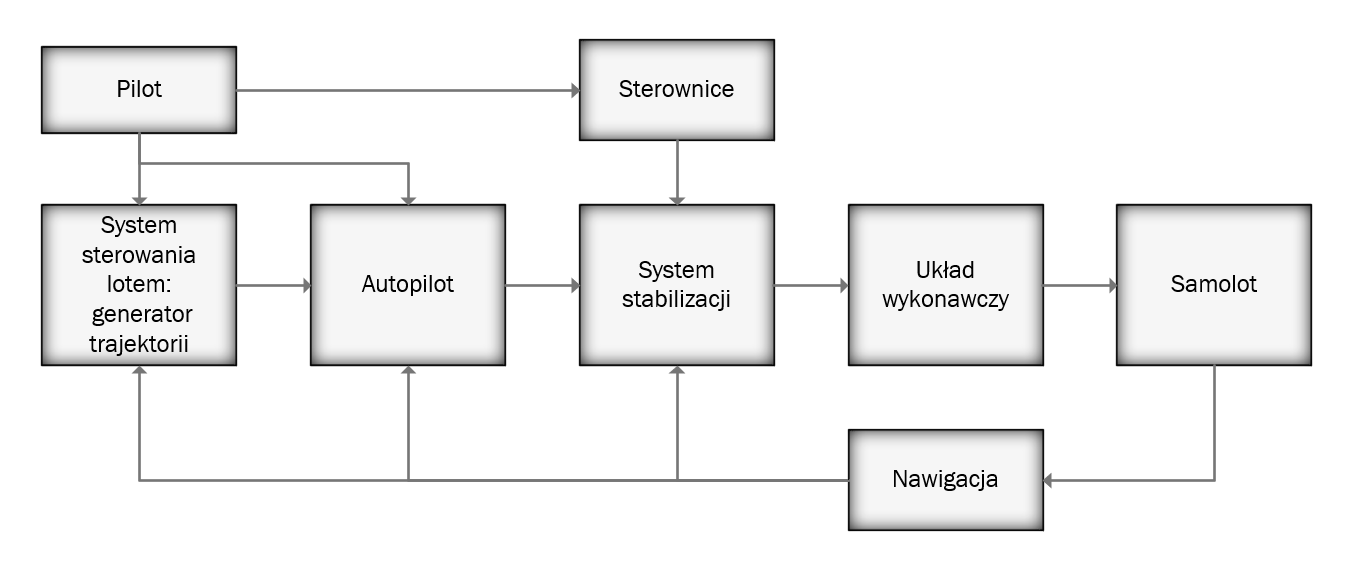
\includegraphics[width=0.9\textwidth]{controller.png}
      	\caption{Układ sterowania BSP.}
      	\label{control_3_stage}
\end{figure}

\begin{figure}[!h]
   	\centering
      	\includegraphics[width=0.9\textwidth]{pid\_cascade.jpg}
      	\caption{Układ sterowania wielowirnikowcem (źródło \cite{energies}).}
      	\label{pid_ladder}
\end{figure}

Ważnym wnioskiem dotyczącym systemów sterowania jest to, że jednym ze sposobów ich projektowania jest kaskadowe łączenie ze sobą kolejnych, elementarnych regulatorów. Umożliwia to opracowanie łatwego w obsłudze interfejsu służącego do ich definiowania i łączenia. Przykładem takie rozwiązania jest toolbox Symulink, będący częścią pakietu MATLAB.

\subsubsection{Regulatory}

W poprzednim rozdziale pokazane zostało, że układ sterowania BSP można zbudować, łącząc ze sobą regulatory jednej wartości. W tym rozdziale zdefiniowane zostanie czym jest regulator, a także przedstawione zostaną przykłady takich regulatorów.\\

Regulator to układ, którego wejście stanowi uchyb $e$, a wyjście $u$ jest podłączone do układów wykonawczych. Celem regulatora jest wystawienie takiego wyjścia, które pozwoli zminimalizować uchyb. Do najprostszych regulatorów zaliczyć można regulatory dwustawne i trójstawne. Regulatory te mogą na wyjście wystawić jedną z~dwóch lub trzech zdefiniowanych wcześniej wartości w zależności od znaku uchybu. Ze względu na swoją prostotę regulatory te mają ograniczony zakres stosowalności. Przykładem takiego regulatora jest prosty termostat. Regulatory te rzadko znajdują zastosowanie w sterowaniu BSP ze względu na nieciągłość wyjścia. Znacznie lepszym podejściem jest wykorzystanie regulatorów o ciągłym sygnale wyjściowym: regulatorów PID i PIFF.\\

\textbf{Regulator PID}  to regulator, w którym wartość wyjściowa jest złożeniem trzech składowych: proporcjonalnej (P - proporcjonalnej), całkowej (I - całkowej) i różniczkowej (D - różniczkowej). Każda z tych składowych pełni określoną rolę w dostosowywaniu działania regulatora do celu sterowania.
Składowa proporcjonalna (P) mierzy aktualną różnicę między wartością rzeczywistą a wartością zadaną (błędu) i dostosowuje sygnał wyjściowy proporcjonalnie do tej różnicy. Im większa różnica, tym większa korekta.
Składowa całkowa (I) bierze pod uwagę całkowity czas trwania błędu. Działa na zasadzie akumulacji błędu w czasie i dostosowuje sygnał wyjściowy w zależności od całkowitej sumy błędów. Pomaga to eliminować błędy statyczne.
Składowa różniczkowa (D) monitoruje tempo zmiany błędu. Działa na zasadzie przewidywania, jak szybko wartość błędu rośnie lub maleje, co pozwala na zapobieganie przesterowaniom i zwiększa stabilność systemu.
Całość regulatora PID można opisać równaniem:
\[
	u(t) = K_p e(t) + K_i \int_{0}^{t} e(\tau) d\tau + K_d \frac{de(t)}{dt},
\]
gdzie: $K_p$, $K_i$ oraz $K_d$ to nastawy regulatora. Dzięki połączeniu trzech składowych regulatory PID pozwalają uzyskać zadaną wartość w krótkim czasie, ze zniwelowaniem efektu przesterowania i błędu statycznego. Poprzez wyzerowanie poszczególnych współczynników uzyskujemy regulatory prostsze np. PD gdy Ki = 0.\\

\begin{figure}[!h]
   	\centering
      	\includegraphics[width=0.8\textwidth]{pid\_graph.png}
      	\caption{Odpowiedź układu z regulatorem PID.}
      	\label{pid_respose}
\end{figure}

Na rysunku (\ref{pid_respose}) przedstawiono odpowiedzi układów z regulatorami P, PI oraz PID. Odpowiedz układu z regulatorem P pokazuje, że samo zastosowanie składowej proporcjonalnej powoduje duże oscylacje, przesterowanie i błąd statyczny. Zastosowanie członu I niweluje błąd statyczny, ale jednocześnie obniża dynamikę układu. Dopiero kompletny regulator PID jest w stanie zapewnić szybkie osiągnięcie wartości ustalonej.\\

W przypadku regulatora PID implementowanego programowo dodatkową trudność stanowi obliczenie pochodnej i całki numerycznej. Wejściowe dane są nierzadko zaszumione, co dodatkowo utrudnia obliczenia. O ile całkowanie nie jest aż tak czułe na szybką zmianę wartości, tak pojedyncza próbka, mocno odbiegająca od rzeczywistej wartości może silnie zaburzyć stabilność układu, gdyż obliczana pochodna będzie niewymiernie duża. Z tego powodu w układach sterowania BSP nierzadko rezygnuje się z członu D \cite{piff} .\\

\textbf{Regulator PIFF} to regulator zbliżony do regulatora PID, w którym człon D został zastąpiony członem sprzężenia w przód (feed-forward). Sprzężenie w przód polega na dodaniu do sygnału wyjściowego odpowiednio przeskalowanej wartości zadanej. W praktyce, w systemach regulacji często występuje pewna zależność między wartością zadaną a wyjściem w stanie ustalonym. Przykładowo, dla samochodu utrzymującego prędkość 60 km/h, silnik musi obracać się z prędkością $2000 \frac{\text{obr}}{\text{min}}$, a~dla prędkości 90 km/h - $3000 \frac{\text{obr}}{\text{min}}$. Ta zależność jest zazwyczaj liniowa. W trakcie jazdy mogą jednak występować różne czynniki, takie jak podmuchy wiatru, które powodują, że rzeczywiste wartości nie zawsze idealnie korespondują z zadanymi. Wykorzystanie członu FF pozwala na zgrubne oszacowanie wyjścia z regulatora, co gwarantuje oczekiwaną odpowiedź systemu. W takim przypadku rola członów P i I ogranicza się do skorygowania ewentualnych błędów. \\

Oprócz przedstawionych nastaw rzeczywiste regulatory posiadają znacznie szerszy zbiór parametrów. Ze względu na ograniczenia sprzętowe wartość wyjściowa z regulatora powinna być ograniczona pomiędzy pewnym minimum i maksimum. Co więcej, jeśli regulator z włączonym członem I przez długi czas nie mógłby osiągnąć zadanej wartości to duża skumulowana wartość w członie całkującym mogłaby doprowadzić do zjawiska Wind-up'u i utraty stabilności. Z tego względu regulatory mają ograniczenie na składową I i specjalne algorytmy zapobiegające temu zjawisku. 

\subsubsection{System nawigacji}

W systemie sterowania jednym z niezbędnych elementów jest układ pomiarowy. Systemy pomiarowe służące do określania parametrów BSP, takich jak położenie i~orientacja, nazywane są systemami nawigacji. System nawigacji montowany jest na pokładzie statku. W trakcie pracy systemy nawigacji gromadzą dane z wielu różnych czujników i na ich podstawie określają interesujące ich parametry. Wiele z tych parametrów wyznaczanych jest pośrednio, z wykorzystaniem odpowiednich przekształceń.\\

W nawigacji lotniczej stosuje się następujące czujniki:
\begin{itemize}
  \item akcelerometry -- dokonują pomiaru przyśpieszeń liniowych,
  \item żyroskopy -- dokonują pomiaru prędkości kątowych,
  \item magnetometry -- dokonują pomiaru pola magnetycznego,
  \item barometry -- dokonują pomiaru ciśnienia statycznego,
  \item rurki spiętrzeniowe -- dokonują pomiaru prędkości względem powietrza,
  \item nawigację satelitarną -- pozwala na oszacowanie pozycji i prędkości.
\end{itemize}

Należy zaznaczyć, że jedynie barometr i nawigacja satelitarna pozwalają uzyskać wyniki w globalnym układzie współrzędnych. Wartości mierzone przez pozostałe czujniki wyrażone są w układzie ruchomym związanym z BSP.\\

Czujniki pomiarowe mają jednak szereg wad. Pomiar nie jest wykonywany natychmiastowo, a wartości mogą być mierzone tylko z określoną częstotliwością nie większą niż częstotliwość maksymalna czujnika. Ze względu na swoją niedoskonałość wartość mierzona przez czujniki obarczona jest błędem losowym i biasem. Aby temu zapobiec w systemach nawigacji, liczba czujników jest nieraz wielokrotnie większa niż to niezbędne. Redundancja nie tylko zabezpiecza przed uszkodzeniem pojedynczego czujnika, ale także pozwala zminimalizować błąd pomiaru poprzez odpowiednie połączenie wyników z różnych czujników. Łączenie pomiaru z wielu czujników w~celu uzyskania kompletnej estymaty parametrów nazywane jest fuzją czujników.\\

Istnieje wiele metod fuzji czujników. Do wyznaczenia orientacji na podstawie pomiarów z akcelerometru, żyroskopu i magnetometru można wykorzystać metodę DCM \cite{dcm} lub metodę filtra komplementarnego \cite{complementary}. Jednak od wielu lat dominującą i uniwersalną metodą określania orientacji jest zastosowanie rozszerzonego filtra Kalmana \cite{ekf_poor}.\\

Filtr Kalmana jest matematyczną metodą estymacji, umożliwiającą efektywne śledzenie stanu dynamicznego systemu oraz filtrację danych pomiarowych obarczonych szumem.
Opiera się na modelowaniu systemu za pomocą równań stanu i~równań pomiarowych. Równania stanu opisują ewolucję stanu systemu w czasie, podczas gdy równania pomiarowe reprezentują zależność między stanem systemu a~danymi pomiarowymi. Matematycznie można to przedstawić w postaci równań:

\[
  x_k = A \cdot x_{k-1} + B \cdot u_k + w_k,
\]

\[
  z_k = H \cdot x_k + v_k,
\]

gdzie:
\begin{itemize}
  \item $x_k$ -- wektor stanu w chwili k, 
  \item $A$ -- macierz przejścia stanu, 
  \item $B$  -- macierz wejścia sterowania, 
  \item $u_k$  -- wektor sterowania, 
  \item $w_k$ -- wektor szumu procesu, 
  \item $z_k$  -- wektor pomiarów w chwili  k, 
  \item $H$ -- macierz pomiaru,
  \item $v_k$ -- wektor szumu pomiarowego.
\end{itemize}

Przedstawione powyżej równania są niejako równaniami stanu układu z dodanym szumem białym. Idea działania filtra opiera się na znalezieniu stanu, który ze statystycznego punktu widzenia jest najbardziej prawdopodobnym, dla zarejestrowanych pomiarów. Wadą powyższego zapisu, podobnie jak w równaniach stanu jest wymóg liniowości. Analogicznie rozwiązaniem tego ograniczenia jest zastosowanie Rozszerzonego Filtru Kalmana (EKF). Równanie stanu EKF prezentują się w następujący sposób:
\[
  x_k =  f \left( x_{k-1},  u_k \right) + w_k,
\]

\[
  z_k = h \left(x_k \right) + v_k,
\]

gdzie:
\begin{itemize}
  \item $ f \left( x_{k-1},  u_k \right)$ -- funkcja stanu, 
  \item $h \left(x_k \right)$ -- funkcja pomiaru.
\end{itemize}

Filtr Kalmana działa w dwóch głównych krokach: predykcji i korekcji. W kroku predykcji prognozowany jest nowy stan systemu oraz jego kowariancja. W kroku korekcji, na podstawie nowych pomiarów, dokonywane jest dostosowanie prognozy, uwzględniając błędy pomiarowe i poprawiając estymację stanu systemu. Filtr zwłaszcza w swojej rozszerzonej wersji stanowi kluczowe narzędzie w dziedzinie sterowania i nawigacji, umożliwiając systemom utrzymanie precyzji pomiarów w~dynamicznych warunkach i poprawę jakości estymacji parametrów systemu.\\

Faza predykcji:
\[
\begin{aligned}
  \hat{x}_k^- & = f(\hat{x}_{k-1}, u_k) \quad \text{(przewidywany stan)}, \\
  P_k^- & = A_k P_{k-1} A_k^T + Q_k \quad \text{(przewidywana kowariancja)},
\end{aligned}
\]

gdzie: $A_k = \frac{\partial f}{\partial x}\Bigr|_{\hat{x}_{k-1}, u_k}$, a $Q_k$ to macierz kowariancji szumu procesu.\\

Faza korekcji:
\[
\begin{aligned}
  &K_k = P_k^- H_k^T (H_k P_k^- H_k^T + R_k)^{-1} \quad \text{(wzmocnienie Kalmana)}, \\
  &\hat{x}_k = \hat{x}_k^- + K_k(z_k - h(\hat{x}_k^-)) \quad \text{(poprawiony stan)}, \\
  &P_k = (I - K_k H_k) P_k^- \quad \text{(poprawiona kowariancja)},
\end{aligned}
\]

gdzie: $H_k = \frac{\partial h}{\partial x}\Bigr|_{\hat{x}_k^-}$, a $R_k$ to macierz kowariancji szumu pomiarowego.
\\

Zastosowanie EKF do nawigacji BSP wymaga określenia składowych wektora stanu i określenia wpływu poszczególnych pomiarów na stan filtra. W fazie predykcji wykorzystane powinny zostać czujniki o dużej częstotliwości próbkowania i te, których pomiary wymagają całkowania. Faza korekcji, która może być wykonywana rzadziej, powinna wykorzystywać czujniki nieposiadające tendencji do kumulowania błędu. W dalszej części rozdziału przedstawiony zostanie zarys zastosowania EKF do określenia pozycji, prędkości i orientacji BSP.\\

Stanem filtru pozwalającego na określenie orientacji BSP w najprostszej wersji może być sam kwaternion orientacji. Filtr startuje z początkową orientacją uzyskaną w~dowolnie inny sposób, np. z metody DCM. Wektorem sterowania filtra jest pomiar z żyroskopu, tj. pomiary prędkości kątowych. W trakcie swojej pracy filtr całkuje kolejne pomiary w celu ustalenia aktualnej orientacji. Faza korekty oparta jest natomiast o akcelerometr i magnetometr. Akcelerometr oprócz właściwego przyśpieszanie BSP rejestruje również wektor przyśpieszenia grawitacyjnego. W czasie, gdy BSP nie wykonuje gwałtownych manewrów, składowa ta dominuje i pozwala skorygować filtr informacją, gdzie znajduje się Ziemia. Analogiczne pomiar z magnetometru, po uwzględnieniu kąta inklinacji i deklinacji pozwala określić kierunek północny.\\

W celu zastosowania filtra do określenia położenia i prędkości minimalnym stanem jest wektor złożony z 3 składowych położenia i 3 składowych prędkości. W fazie predykcji wykorzystywane są dane z przyśpieszeniomierza, które należy wstępnie obrócić do układu globalnego i pozbawić składowej związanej z przyśpieszeniem grawitacyjnym. Całkując jednokrotnie przyśpieszenia, uzyskujemy prędkości, a dwukrotnie położenie. W fazie korekcji wykorzystuje się pomiary z nawigacji satelitarnej i barometru. Nawigacja satelitarna ma relatywnie małą częstotliwość próbkowania, ale pozwala w sposób bezwzględny określić pozycję BSP. Wiele systemów nawigacji satelitarnej wykorzystuje również efekt Dopplera do określenia prędkości odbiornika. Barometr natomiast pozwala na oszacowanie wysokości, porównując zmierzoną wartość do wartości referencyjnej. Wysokość określana na podstawie wskazań barometru, nazywana wysokością barometryczną, do dziś znajduje zastosowanie w~lotnictwie.\\

Zarys przedstawiony powyżej stanowi jedynie podstawowy wariant wykorzystywany EKF w nawigacji. W rzeczywistych zastosowaniach stan filtra jest znacznie rozszerzony, uwzględniając w sobie m.in. biasy czujników oraz estymatę warunków atmosferycznych, jak np. prędkość i kierunek wiatru, a pomiary z czujników są wstępnie filtrowane.


